\chapter{Literature Review}
\label{cha:2}

\section{Identity-Based Encryption}
Shamir~\cite{art:Shamir84} already proposed a concept of identity-based cryptography in 1984. In identity-based cryptography any string can be a valid public key for encryption or signature schemes thereby eliminating the need for digital certificates. Identity-based cryptography proves to be particularly elegant if the public key is related to an attribute that uniquely identifies the identity of the user like an e-mail address, an IP address or a telephone number. Consequently, identity-based cryptography reduces system complexity and the cost for establishing and managing the Public Key Infrastructure~(PKI)~\cite{art:BaekNSS04}. 


\subsection{Definition}
A generic Identity-Based Encryption (IBE) scheme is composed of four probabilistic polynomial time algorithms~\cite{art:BonehF01}:
\begin{description}
    \item[\texttt{IBE.Setup($1^k$)}] On input of a security parameter $k$, outputs a master secret $s_k$ and public parameters $params$.
    \item[\texttt{IBE.Extract($params, s_k, \id{}$):}] Takes public parameters $params$, the master secret $s$, and an \id{} as input and returns the private key $s_{\id{}}$ corresponding to the identity \id{}.
    \item[\texttt{IBE.Encrypt($params, \id{}, m$):}] Returns the encryption $c$ of the message $m$ on the input of the public parameters $params$, the \id{}, and the arbitrary length message $m$.
    \item[\texttt{IBE.Decrypt($s_{\id{}}, c$):}] Decrypts the ciphertext $c =$ \texttt{IBE.Encrypt}($params, \id{}, m$) back to the message $m$ on input of the secret key $s_{\id{}}$ corresponding to the receiving identity \id{}.
\end{description}

\begin{figure}[ht]
    \begin{center}
    \scalebox{0.78}{
        \begin{tikzpicture}[auto, node distance=1mm, align=center,
            block/.style={rectangle,text width=6em,text centered,minimum height=11mm},
            line/.style={draw,very thick, ->},
            line2/.style={draw,very thick, <->},
            leg/.style={text centered},
            ]
            %\draw[help lines] (-6,-5) grid (8,3);
            \path
                % Images
                (-0.5,3) node [block] (pkg) {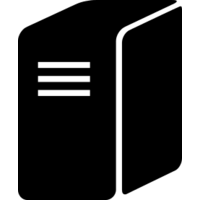
\includegraphics[scale=0.2]{img/pkg.png}}
                (-4,0) node [block] (alice) {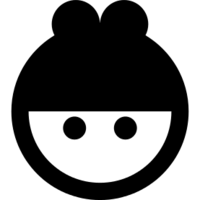
\includegraphics[scale=0.2]{img/alice.png}}
                (4,0) node [block] (bob) {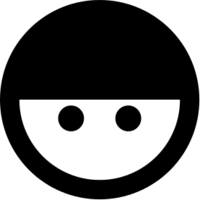
\includegraphics[scale=0.2]{img/bob.png}}
                % Text
                (-0.5, 0.5) node [leg, color=orange] (c) {$c$}
                (1.5, 1.2) node [leg] (id_bob) {$s_{\id{Bob}}$}
                (3.5,2) node [leg] (bob_authenticates) {4. Bob authenticates}
                ;
                
       \node[below=of pkg] {\textbf{PKG}};
       \node[below=of alice] {\textbf{Alice} \\ 3. $c \leftarrow $\texttt{IBE.Encrypt($params, \id{Bob}, m$)}};
       \node[below=of bob] {\textbf{Bob} \\ 6. $m \leftarrow $\texttt{IBE.Decrypt($s_{\id{Bob}}, \id{Bob}$)}};
       \node[above=of pkg,align=left] {
               1. $\left< s_k, params \right> \leftarrow $\texttt{IBE.Setup($1^k$)} \\
               2. publish $params$ \\
               \\
               5. $s_{\id{Bob}} \leftarrow $\texttt{IBE.Extract($params, s_k, \id{Bob}$)}
               };
       \begin{scope}[every path/.style=line]
        \path[color=orange] (alice.east) -- (bob.west);
        \path (2.8,1) -- (1,2.2);
        \path (0.9,2.1) -- (2.7,0.9);
       \end{scope}


        \end{tikzpicture}
    }
    \end{center}
    \caption{Generic identity-based encryption scheme. The orange arrow denotes an insecure channel that can be eavesdropped.}
    \label{fig:generic_ibe_scheme}
\end{figure}

These generic algorithms are best explained using Figure~\ref{fig:generic_ibe_scheme}. A trusted Public Key Generator (PKG) generates a master secret key $s_k$ and public parameters $params$ on input of the security parameter $k$. Next, the PKG publishes the public parameters $params$ while storing $s_k$ preferably in encrypted fashion on a local disk. When Alice wants to send a message $m$ to Bob, it suffices for her to know the public parameters $params$ and his id $\id{Bob}$ uniquely identifying Bob. Alice encrypts the message to a ciphertext $c$ that is sent over to Bob. On receipt of the ciphertext, Bob authenticates to the PKG over a secure channel to request his secret key $s_{\id{Bob}}$. Next, the PKG generates the secret key $s_{\id{Bob}}$ corresponding to Bob's identity $\id{Bob}$ on input of the master secret key $s_k$, Bob's id $\id{Bob}$ and public parameters $params$. Subsequently, the PKG sends $s_{\id{Bob}}$ back again over a secure channel. Finally, Bob has all the required information to decrypt the ciphertext $c$ to its original plaintext message $m$.

\subsection{Advantages and Drawbacks of IBE}
Note that it is important that the PKG can be fully trusted as it will generate all the secret keys $s_{\id{}}$ in the system. Referring to Figure~\ref{fig:generic_ibe_scheme}, a malicious PKG server could use this information to start eavesdropping on the insecure channel between Alice and Bob while decrypting all ciphertexts that are being sent over. The undesired property that private keys have to be shared with a trusted third party is often called \textit{key escrow} in literature.

Another drawback from the scheme in Figure~\ref{fig:generic_ibe_scheme} is that keys can not be revoked in the system. However, Bob's secret key $s_{\id{Bob}}$ can still get compromised if he is careless with the storage of his secret key. In fact, a lot of research has been done in literature on the revocation of IBE keys~\cite{art:BoldyrevaGK12,art:BonehDTW01,art:HanaokaHSI05,art:LibertQ03}. Key revocation often requires additional infrastructure that complicates the elegancy of the currently proposed IBE scheme. As a matter of fact, the major drawback of revoking Bobs key is that Bob can no longer receive encrypted messages because his public key is part of his identity. Therefore, a pragmatic solution to this issue could be to append expiration dates to the public keys. Consequently, public keys will only be valid for a limited amount of time thereby restricting the damage that could be done with a compromised secret key~\cite{art:BonehF01}.

The scheme from Figure~\ref{fig:generic_ibe_scheme} has some desired properties as well. For starters, only one PKG suffices to realise the system, which relaxes expensive requirements on the public key infrastructure. Furthermore, once the PKG has successfully delivered all the secret keys in the system, it can go offline as the scheme does not require any future interactions between the PKG and the users in the system.

Another useful property of an IBE scheme is that Bob does not need to subscribe to a hierarchy of Certification Authorities neither a chain of trust before Alice can start sending him messages. In this way, the possibility to send encrypted messages becomes inherently part of any system in which the users are assigned unique identifiers. This is particularly useful in systems where the majority of the users has no knowledge about cryptographic primitives.  Users do no longer need to generate a key pair neither subscribe to a third party infrastructure. It suffices to recall how their connections can be uniquely identified in the system to know their public keys.

\subsection{Security of IBE}
A cryptographic scheme should meet two properties in order to be of practical use. First, the scheme should be consistent, i.e. decryption reverses encryption. Second, the scheme should be secure. The definition of security is more subtle as different levels of security can be defined. In IBE \textit{indistinguishability under chosen plaintext attack} (IND-CPA) and \textit{indistinguishability under chosen ciphertext attack} (IND-CCA) are often considered. Anonymity of the encryption scheme is an additional property of the scheme that is often desired~\cite{thesis:Alfredo08}.

\subsubsection{Indistinguishability Under Chosen Plaintext Attack}
\subsubsection{Indistinguishability Under Chosen Ciphertext Attack}
\subsubsection{Anonymous Identity-Based Encryption}


\subsection{Evolution of IBE}
Although Shamir easily constructed an identity-based signature scheme based on RSA in 1984, the use case of IBE remained an open problem until the introduction of bilinear maps. In~\cite{art:BonehF01} Boneh and Franklin propose the first practically usable IBE scheme based on the Weil pairing. However, the security proof in~\cite{art:BonehF01} still relies on the random oracle assumption. Canetti et al.~\cite{art:CanettiHK03} succeed in proposing a secure IBE scheme without having to rely on the random oracle model. However, the attacker model in~\cite{art:CanettiHK03} requires the adversary to declare which identity it will target, therefore the scheme in~\cite{art:BonehF01} is considered more secure as attackers can adaptively choose the targeted identity. Gentry~\cite{GentryRandomOracles} proposes a more efficient alternative to this scheme without random oracles while achieving shorter public parameters. 



\section{Broadcast Encryption}

\subsection{Definition}

\subsection{Anonymous Broadcast Encryption}

\subsection{Outsider-Anonymous Broadcast Encryption}


\section{Secret Sharing}

\subsection{Definition}
\begin{defn}[Secret Sharing Scheme]
\label{def:secret_sharing_scheme}
 A \textit{Secret Sharing Scheme} is a cryptographic scheme that divides a secret $S$ into $n$ pieces of data $S_1, \ldots, S_n$ called \textit{shares}. Shares are distributed over $n$ different parties called \textit{shareholders} such that specific subsets of the distributed shares allow reconstruction of the original secret $S$.
\end{defn}

\begin{defn}[Threshold scheme]
\label{def:threshold_scheme}
 A $\left( t, n \right)$ \textit{threshold scheme} $\left( t \leq n \right)$ is a secret sharing scheme by which a trusted party securely distributes $n$ different shares $S_i$ to $n$ different parties $P_i$ for $1 \leq i \leq n$ such that any subset of $t$ or more different shares $S_i$ easily allows to reconstruct the original secret $S$. Knowledge of $t-1$ or less shares is insufficient to reconstruct the original secret $S$.
\end{defn}

\begin{defn}[Perfect threshold scheme]
\label{def:threshold_scheme}
 A $\left( t, n \right)$ threshold scheme is said to be \textit{perfect} if no subset of fewer than $t$ shareholders can derive any partial information in the information theoretic sense about the original secret $S$ even with infinite computational resources.
\end{defn}

\subsection{Shamir Secret Sharing}
In 1979, both Shamir~\cite{art:Shamir79} and Blakley~\cite{art:Blakley79} independently found an algorithm achieving perfect threshold secret sharing. Shamir's solution was based on polynomial interpolation while Blakley's algorithm relied on finite geometries. Blakley secret sharing uses more bits than necessary as it describes multidimensional planes. In contrast, Shamir secret sharing requires as many bits for each share as the length of the original secret. Therefore Shamir secret sharing has gained more popularity in both research communities and in practical implementations.

\begin{algorithm}
\caption{Shamir's $\left( t, n \right)$ threshold scheme~\cite{book:handbook_of_applied_cryptography} }
\label{alg:shamirs_threshold_sheme}
 \textbf{Goal}: A trusted party $T$ distributes shares of a secret $S$ to $n$ parties.
 
 \textbf{Result}: If a subset of at least $t$ out of $n$ shareholders collaborates, they can reconstruct the original secret $S$.
 \begin{enumerate}
  \item \textit{Setup} The trusted party T begins with a secret integer $S \geq 0$ it wishes to distribute among $n$ parties
   \begin{enumerate}
    \item T chooses a prime $p > \max \left( S, n \right)$ and defines $a_0 = S$
    \item $T$ selects $t-1$ random, independent coefficients $a_1, \ldots, a_{t-1}, 0 \leq a_j \leq p-1$ defining the random polynomial over $\mathcal{Z}_p$, $f \left( x \right) = \sum^{t-1}_{j=0} a_j x^j$
    \item $T$ computes $S_i = f \left( i \right) \bmod p, 1 \leq i \leq n$ and securely transfers the share $S_i$ to shareholder $P_i$, along with a public index $i$.
   \end{enumerate}
   \item \textit{Reconstruction} Any group of $t$ or more shareholders pool their shares. Their shares provide $t$ distinct points $\left( x, y \right) = \left( i, S_i \right)$ allowing computation of the coefficients $a_j, 1 \leq j \leq t-1$ of $f \left( x \right)$ by Lagrange interpolation. The secret is recovered by calculating
 \begin{equation*}
  f \left( 0 \right) = \sum^t_{i=1}y_i \prod_{1 \leq j \leq t, j \neq i} \frac{x_j}{x_j-x_i} = S
 \end{equation*}
 \end{enumerate}
\end{algorithm}

The idea behind Shamir secret sharing is elegant in its simplicity. Any polynomial $f \left( x \right)$ of degree $t-1$ is uniquely defined by $t$ points lying on the polynomial. For example, it is possible to draw only one straight line between 2 different coordinates, a quadratic is fully defined by 3 different coordinates and so on. If the trusted party randomly generates a polynomial of degree $t-1$ it suffices to securely distribute one of $n$ different coordinates on the curve to each party $P_i, 0 \leq i \leq n$. A subset of at least $t$ different shareholders has to collaborate in order to reconstruct the original polynomial by interpolation. For security reasons the polynomial $f \left( x \right)$ is calculated in a finite field modulo a large prime number $p$. The complete mechanism of Shamir's threshold scheme can be found in Algorithm~\ref{alg:shamirs_threshold_sheme}. The mechanism behind reconstruction in Algorithm~\ref{alg:shamirs_threshold_sheme} is explained because the coefficients of an unknown polynomial $f \left( x \right)$ of degree less than $t$, defined by points $\left( x_i, y_i \right), 1 \leq i \leq t$ are given by the Lagrange interpolation formula

\begin{equation*}
 f \left( x \right) = \sum^t_{i=1}y_i \prod_{1 \leq j \leq t, j \neq i} \frac{x-x_j}{x_i-x_j}
\end{equation*}
A proof of this formula is omitted but can be found in~\cite{site:proofwiki_lagrange}.

\subsection{Verifiable Secret Sharing}
Verifiable secret sharing~\cite{art:ChorGMA85} tries to ensure the participating parties that their received shares are consistent by providing a verification mechanism. This verification mechanism can either detect an unfair dealer during setup or participants submitting incorrect shares during the reconstruction phase. The first verifiable secret sharing schemes were \textit{interactive}, i.e. interaction between shareholders and the trusted party was required to verify their shares. In \textit{non-interactive verifiable secret sharing} only the trusted party is allowed to send messages to the future shareholders. Shareholders can not communicate with each other neither can they send messages back to the trusted party. Non-interactive verifiable secret sharing is preferred over interactive alternatives as their is no chance of shareholders accidentally leaking too much information.

Popular verifiable secret sharing schemes are Feldman's scheme~\cite{art:Feldman87} and Benaloh's scheme~\cite{art:Benaloh86a}. No further details are given as a basic notion of verifiable secret sharing suffices for the remainder of this text.

\section{Distributed Key Generation}

\section{Conclusion}
The final section of the chapter gives an overview of the important results of this chapter. This implies that the introductory chapter and the concluding chapter don't need a conclusion.

\lipsum[66]

%%% Local Variables: 
%%% mode: latex
%%% TeX-master: "thesis"
%%% End: 
